\section{Deep Learning}\label{sec:hw-nas:dl}

    A neural network architecture typically consists of a series of linked operations or blocks of operations that, when working together, enable the model to process input data, learn patterns and representations and produce corresponding predictions.
    
    In this section, we'll cover the primitive operations upon which neural networks are built, and the classic building blocks that are created through combinations of these operations. These blocks make it easier to design neural networks by using them repeatedly.
    
    Throughout this section, the computational cost of an operation or a block will be measured in \gls{abb:flops}, while the memory usage  dictated through \gls{abb:macs}. The notation used will be as follows:
    .

    \begin{table}[hbt!]
        \begin{tabularx}{\textwidth}{@{}XX@{}}
        \toprule
          $n$ & batch size \\
          $c_i$ & input channels \\
          $c_o$ & output channels \\
          $k_h$ & kernel height \\
          $k_w$ & kernel width \\
          $h_i$ & input tensor height \\
          $w_i$ & input tensor width \\
          $h_o$ & output tensor height \\
          $w_o$ & output tensor width \\
        \bottomrule
        \end{tabularx}
    \end{table}


    
    \subsection{Primitive Operations}
            
        \subsubsection{Fully connected layer}
        
            A fully connected layer, also referred to as a dense layer or a linear layer, serves as a foundational layer in neural networks, connecting every single input neuron to all output neurons as described in~\Cref{fig:hw-nas:dl:dense}.
            
            \begin{table}[hbt!]
                \caption{Fully connected layer}
                \begin{tabularx}{\textwidth}{@{}XX@{}}
                \toprule
                  Input tensor  &  $X(n,c_i)$\\
                  Weights tensor  &  $W(c_o, c_i)$\\
                  Output tensor &  $Y(n,c_o)$\\
                  \gls{abb:macs}  &  $n.c_o.c_i$\\
                  \gls{abb:flops} &  $2.n.c_o.c_i$\\
                \bottomrule
                \end{tabularx}
            \end{table}

            \begin{figure}[hbt!]
                \begin{center}
                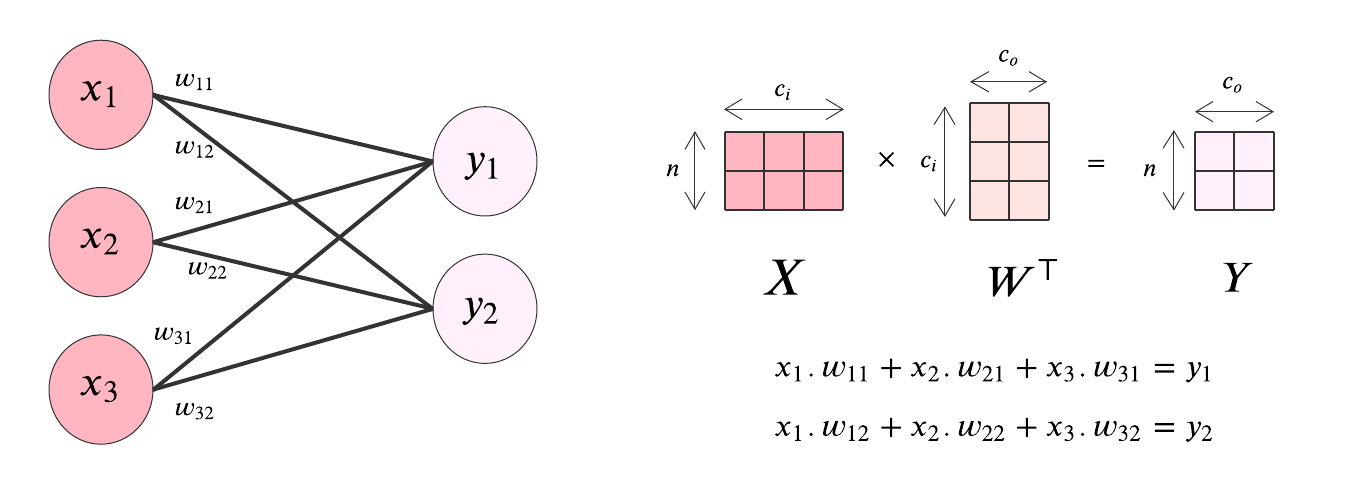
\includegraphics[width=.9\textwidth]{assets/images/dense.png}
                \end{center}
                \caption{Fully connected layer}%
                \label{fig:hw-nas:dl:dense}
            \end{figure}
            
        \subsubsection{Convolution layer}
            A convolution layer performs a mathematical operation called convolution on input data. It involves sliding kernels (also referred to as filters), which have a small receptive field, over the input data to extract features and capture spatial patterns.
            
            \begin{table}[hbt!]
                \caption{Convolution layer}
                \begin{tabularx}{\textwidth}{@{}XX@{}}
                \toprule
                  Input tensor  &  $X(n, c_i,  h_i, w_i)$\\
                  Weights tensor  &  $W(c_o, c_i, k_h, k_w)$\\
                  Output tensor  &  $Y(n, c_o, h_o, w_o)$\\
                  \gls{abb:macs}  &  $n.c_o.c_i.k_h.k_w.h_o.w_o$\\
                  \gls{abb:flops} &  $2.n.c_o.c_i.k_h.k_w.h_o.w_o$\\
                \bottomrule
                \end{tabularx}
            \end{table}
            
            
        \subsubsection{Grouped Convolution layer}
        
            To reduce computation and the number of parameters needed by the convolution layer, grouped convolution was introduced in AlexNet~\cite{conv} to distribute the model over multiple GPUs. Instead of applying the same kernels to the entire input, grouped convolution divides the input channels into $g$ groups and applies separate sets of kernels to each group independently.
            
            \begin{table}[hbt!]
                \caption{Grouped convolution layer}
                \begin{tabularx}{\textwidth}{@{}XX@{}}
                \toprule
                  Input tensor  &  $X(n, c_i,  h_i, w_i)$\\
                  Weights tensor  &  $W(g, \frac{c_o}{g} , \frac{c_i}{g} , k_h, k_w)$\\
                  Output tensor  &  $Y(n, c_o, h_o, w_o))$\\
                  \gls{abb:macs}  &  $n\times \frac{c_o\times c_i \times k_h \times k_w \times h_o \times w_o}{g}$\\
                  \gls{abb:flops} &  $2 \times n \times \frac{c_o \times c_i \times k_h \times k_w \times h_o \times w_o}{g}$\\
                \bottomrule
                \end{tabularx}
            \end{table}
            
            
        \subsubsection{Depthwise convolution layer}
                
            Depthwise convolution~\cite{mobilenet} is a special case of grouped convolution, where the number of groups $g$ is equal to the number of input channels $c_i$. The layer applies a single filter to each input channel separately, capturing information independently across channels, and then stacks the results, as illustrated in~\Cref{fig:hw-nas:dl:depthwise}. This leads to a notable reduction in computational cost and model parameters, making it more suitable for mobile phones and resource-constrained devices.
            
            \begin{table}[hbt!]
            \caption{Depthwise convolution layer}
            \begin{tabularx}{\textwidth}{@{}XX@{}}
            \toprule
              Input tensor &  $X(n, c_i,  h_i, w_i)$\\
              Weights tensor &  $W(c_o, k_h, k_w)$\\
              Output tensor  &  $Y(n, c_o, h_o, w_o)$\\
              \gls{abb:macs}  &  $n.c_o.k_h.k_w.h_o.w_o$\\
              \gls{abb:flops} &  $2.n.c_o.k_h.k_w.h_o.w_o$\\
            \bottomrule
            \end{tabularx}
            \end{table}

              
            \begin{figure}[hbt!]
                \begin{center}
                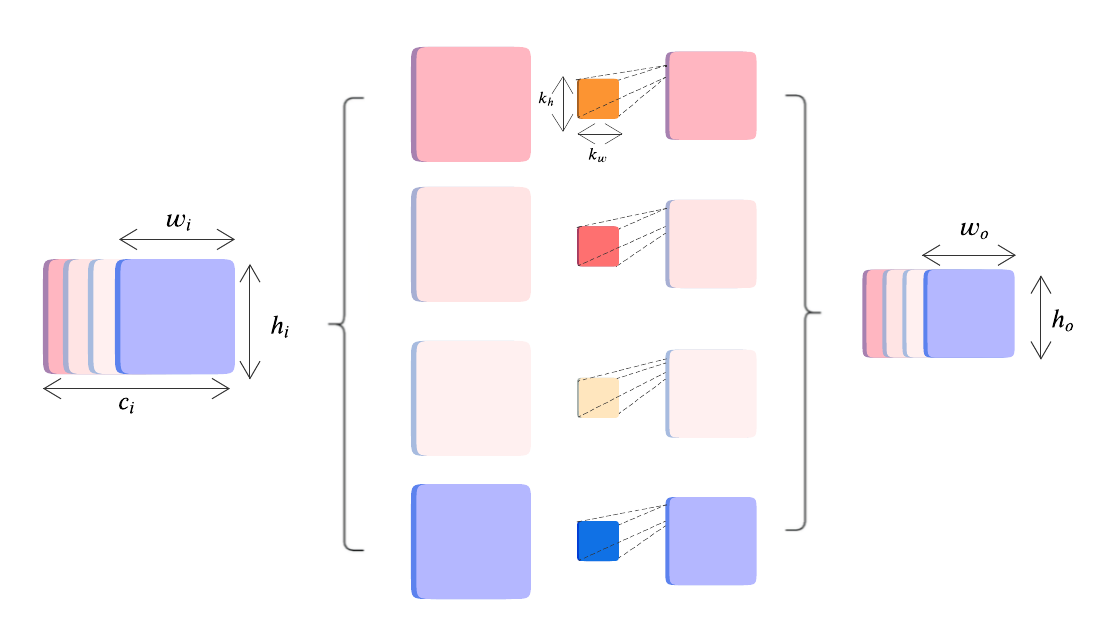
\includegraphics[width=.9\textwidth]{assets/images/depthwise.png}
                \end{center}
                \caption{Depthwise Convolution Layer}%
                \label{fig:hw-nas:dl:depthwise}
            \end{figure}
            

            
        \subsubsection{Pointwise convolution layer}
            A pointwise convolution layer~\cite{pointwise} is a convolution layer with 1 \times 1 kernels ($k_w = k_h = 1$). It is used for managing the number of channels, i.e., changing the dimensionality of another operation's input, and also for creating channel-wise dependencies and exchanging information between groups that have been separately computed by depthwise or grouped convolution. The layer's working is presented in~\Cref{fig:hw-nas:dl:pointwise}.

            \begin{table}[hbt!]
            \caption{Pointwise convolution layer}
            \begin{tabularx}{\textwidth}{@{}XX@{}}
            \toprule
              Tensor &  Shape \\
              Input tensor &  $X(n, c_i,  h_i, w_i)$\\
              Weights tensor &  $W(c_o, 1, 1)$\\
              Output tensor  &  $Y(n, c_o, h_o, w_o)$\\
              \gls{abb:macs}  &  $n.c_o.h_o.w_o$\\
              \gls{abb:flops} &  $2.n.c_o.h_o.w_o$\\
            \bottomrule
            \end{tabularx}
            \end{table}

              \begin{figure}[hbt!]
                \begin{center}
                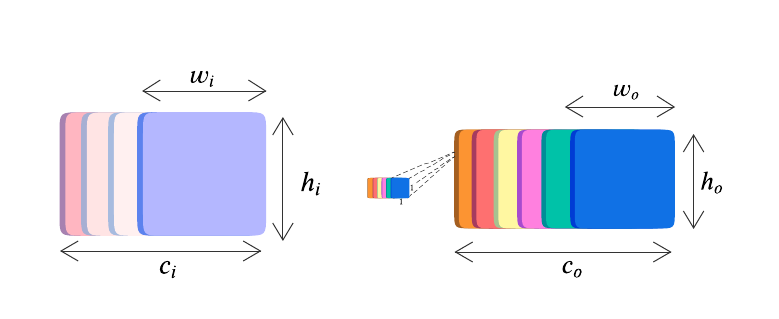
\includegraphics[width=.9\textwidth]{assets/images/pointwise.png}
                \end{center}
                \caption{Pointwise Convolution Layer}%
                \label{fig:hw-nas:dl:pointwise}
            \end{figure}
        
        
        \subsubsection{Dilated convolution layer}
            A dilated convolution layer~\cite{dilated}, also referred to as an atrous convolution layer, is a type of convolution that involves pixel skipping to enlarge the receptive field of kernels without increasing the number of parameters. This is achieved by expanding the kernel and inserting holes between its consecutive elements. The dilation factor $l$ indicates how much the kernel is widened, resulting in the skipping of $l-1$ pixels in the kernel. A standard convolution is a dilated convolution with a dilation factor of $1$.

        \subsubsection{Pooling layer}
            While convolution layers extract features from data, pooling layers consolidate the extracted features. A pooling layer is a downsampling operation typically added after convolution layers to reduce their output dimensions and minimize the number of parameters and computations. Pooling layers also contribute to making representations invariant to small translations of the input; that is, if the input is slightly translated, most of the pooled output values remain unchanged~\cite{dlbook}. The pool size refers to the dimensions of the window sliding over the feature map to apply pooling.

            There are two types of pooling commonly used:
            \begin{itemize}
                \item  \textbf{Max pooling:} Selects the maximum value from each pool, preserving the most prominent features of the feature map. It is the most commonly used type.
                \item \textbf{Average pooling:} Computes the average of the pool, preserving the average values of features in the feature map.
            \end{itemize}

        \subsubsection{Self-Attention}
            Self-attention layer is a central mechanism in the transformer architecture~\cite{attention} that identifies dependencies and relations within input sequences. It contextually encodes the input sequence embeddings by calculating soft weights for each word’s embedding within the context window. It operates by applying linear transformations on the input sequence and transforming them into Query, Key and Value vectors. A weighted sum of the values is calculated based on the similarity between the Query and key vectors, which is then passed along with the original input through a \gls{abb:ffnn} to get the final output.
    
    
    \subsection{Classic building blocks}
    
        A building block is a modular unit linking multiple primitive operations to achieve a balance between accuracy and computational efficiency. These interconnected layers form a structure that will serve as a fundamental component in a model architecture.
    
    
        \subsubsection{Bottleneck Residual Block}
            
            The bottleneck block was introduced as part of the ResNet~\cite{resnet50} architecture. It consists of three layers: a 1x1 convolution ($\text{conv}$ 1x1), a 3x3 convolution ($\text{conv}$ 3x3), and another 1x1 convolution. The pointwise layers are employed to create a bottleneck containing the $\text{conv}$ 3x3 operation. The block architecture is illustrated in~\Cref{fig:hw-nas:dl:bottleneck}.
            
            By comparing computational and memory usage costs, it is observed that $\text{conv}$ 3x3 is nine times more computationally expensive than $\text{conv}$ 1x1. So, in this block, rather than directly feeding a large input through $\text{conv}$ 3x3, the block first reduces the input's channel dimension by a factor of $4$ using a pointwise layer. Following this, the $\text{conv}$ 3x3 operation is performed with a smaller input, and then the number of channels of its output is expanded back using another pointwise layer.

            
            \begin{figure}[hbt!]
                \begin{center}
                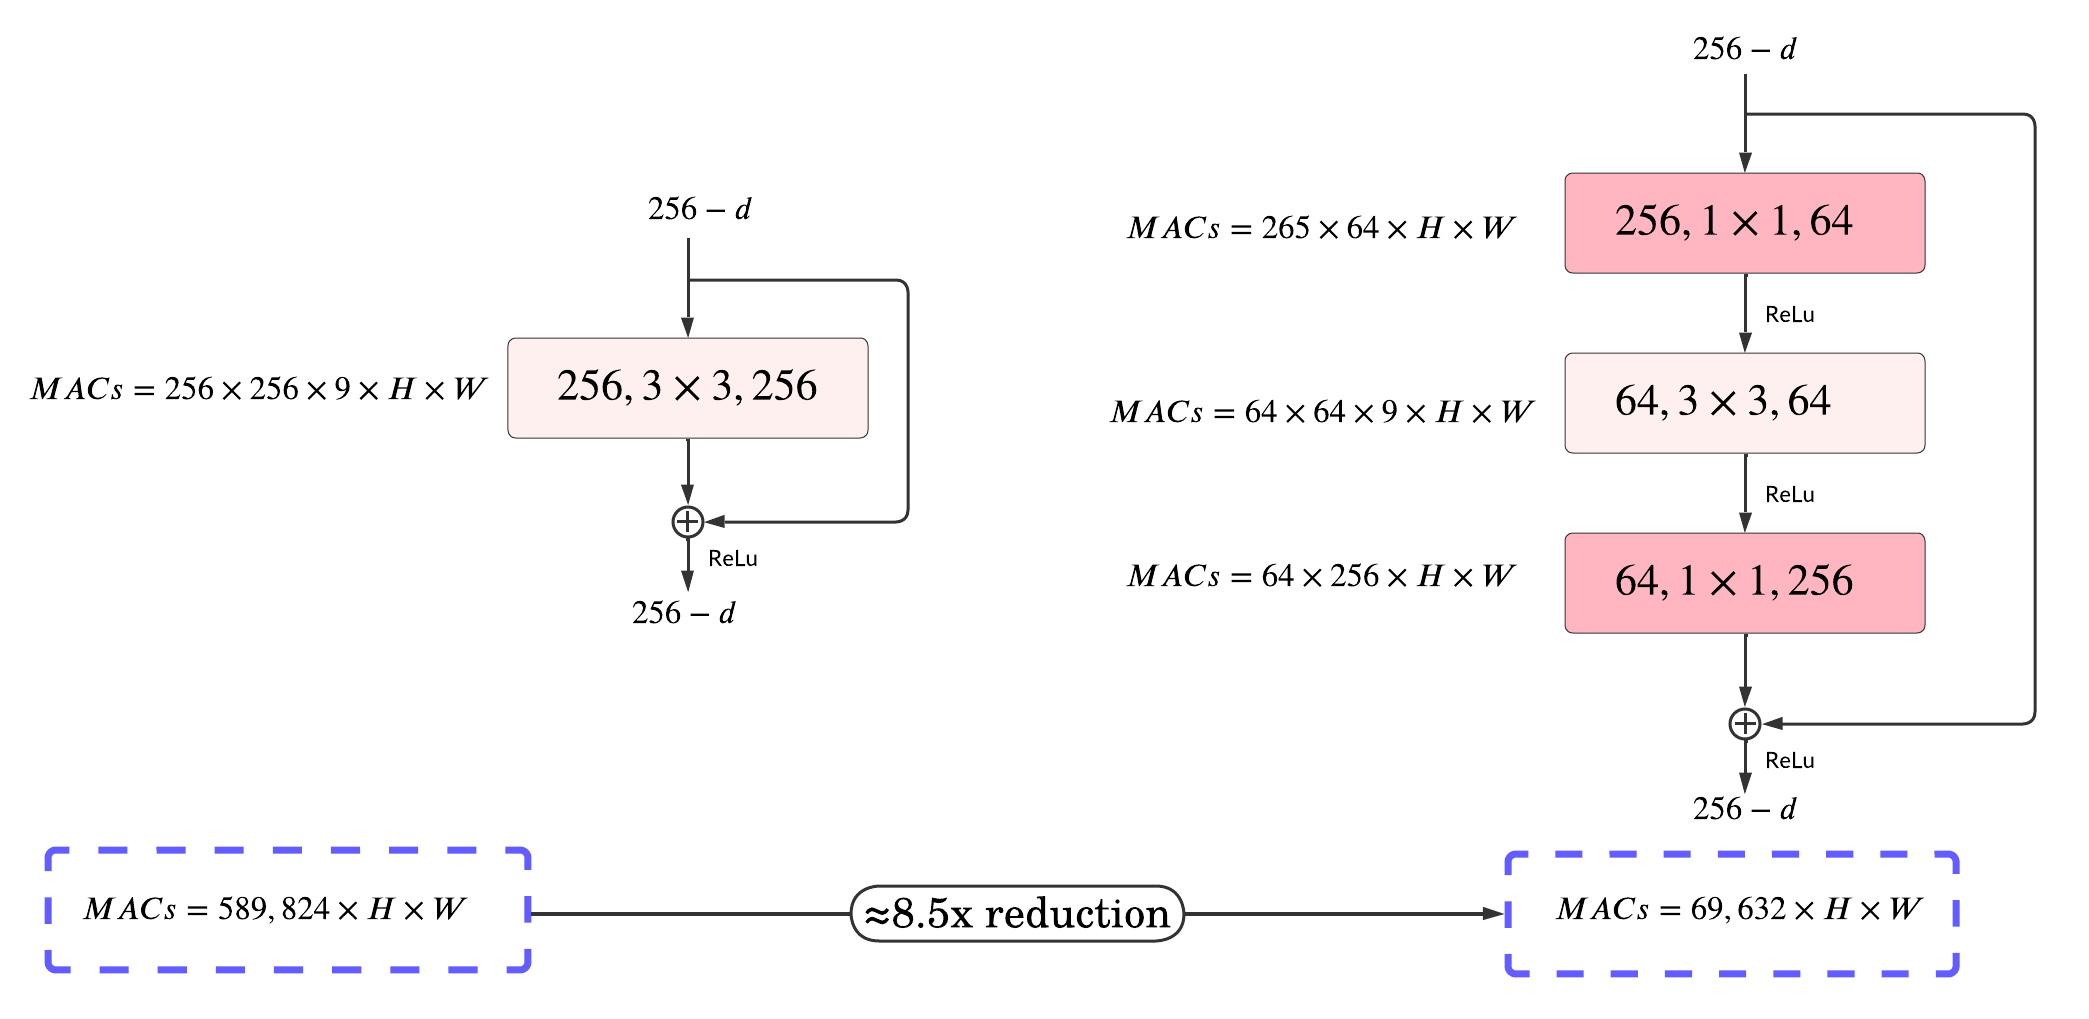
\includegraphics[width=.9\textwidth]{assets/images/bottleneck.png}
                \end{center}
                \caption{Bottleneck Residual Block}%
                \label{fig:hw-nas:dl:bottleneck}
            \end{figure}
    

    
        \subsubsection{ResNeXt Block}
        
            The ResNeXt block~\cite{resnext} is a bottleneck residual block that replaces the convolution operations with grouped convolutions and then aggregates the results to implement a "split-transform-merge" strategy, as presented in~\Cref{fig:hw-nas:dl:resnext}. The group factor in this context is called cardinality $C$.
            
            So in ResNeXt, instead of performing a $\text{conv}$ 3\times3 operation with 128 input channels and 128 output channels, 32 $\text{conv}$ 3\times3 operations are performed with 4 input channels and 4 output channels each (~\Cref{fig:hw-nas:dl:resnext}). This is more efficient because the 32 smaller convolutions are independent.

            \begin{figure}[hbt!]
                \begin{center}
                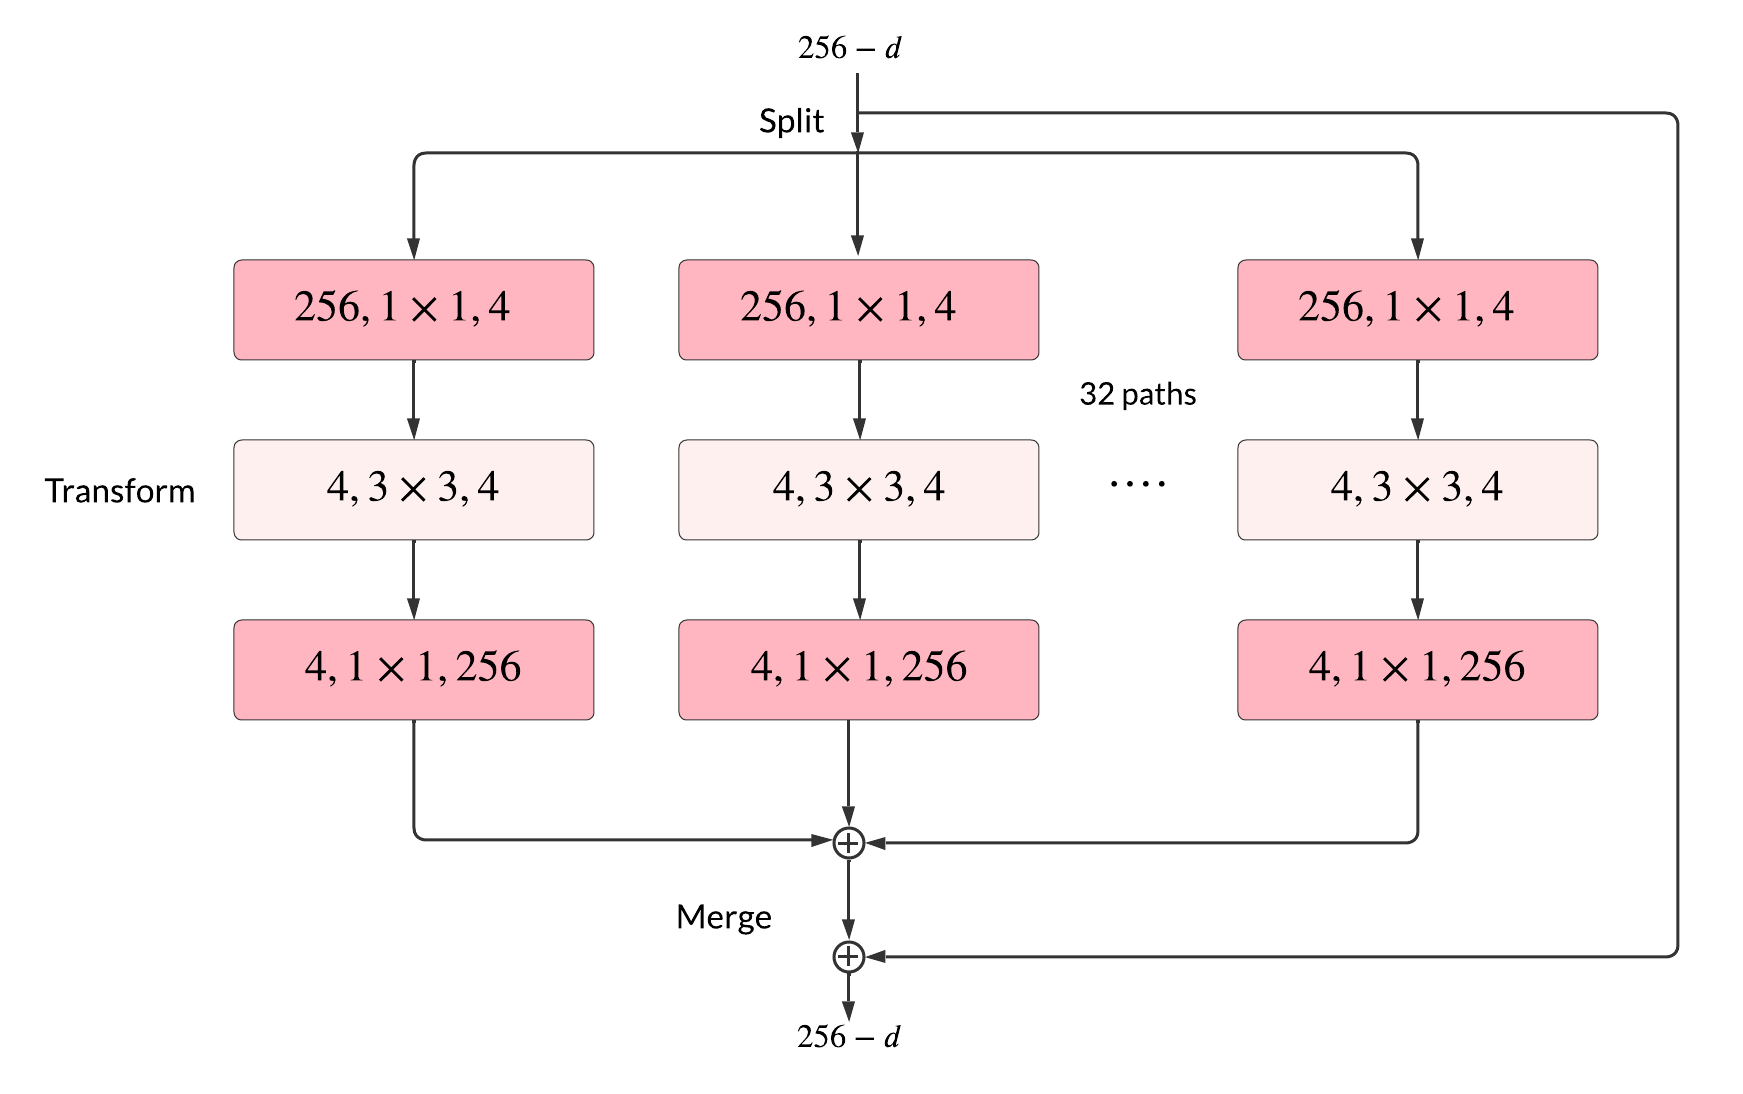
\includegraphics[width=.9\textwidth]{assets/images/resnext.png}
                \end{center}
                \caption{ResNeXt block}%
                \label{fig:hw-nas:dl:resnext}
            \end{figure}
            
            
        
        \subsubsection{Depthwise-Separable Block}
        
            The Depthwise Separable Convolution Block~\cite{mobilenet}, in contrary to a standard convolution layer, splits the channel-wise and spatial-wise computation into two steps. First, a depthwise convolution is applied to capture spatial information, and then a pointwise convolution is applied to exchange the captured information across different channels, as can be seen in~\Cref{fig:hw-nas:dl:dwsep}.

            \begin{figure}[hbt!]
                \begin{center}
                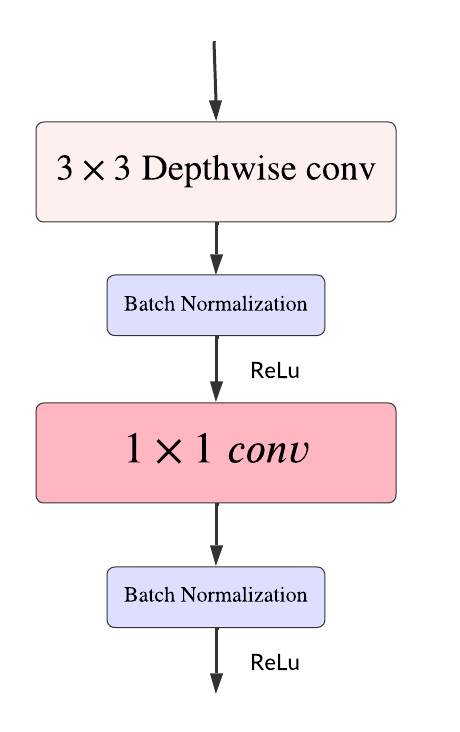
\includegraphics[width=.3\textwidth]{assets/images/depthwise_sep.png}
                \end{center}
                \caption{Depthwise-Separable Block}%
                \label{fig:hw-nas:dl:dwsep}
            \end{figure}
                    
            
        \subsubsection{Inverted Bottleneck Residual Block}
            The inverted bottleneck block~\cite{mobilenetv2}, also referred to as MBConv, is similar to the bottleneck block but uses depthwise 3x3 convolution instead of standard one. However, it is inverted, i.e. it has a expand → depthwise conv 3x3 → reduce structure instead of the standard reduce → depthwise conv 3x3 → expand structure.  This inversion is due to the low capacity of depthwise convolution, so to make up for the loss of model capacity, the number of channels is increased before feeding to the depthwise conv 3x3 operation. This is illustrated in~\Cref{fig:hw-nas:dl:inverted}.

            \begin{figure}[hbt!]
                \begin{center}
                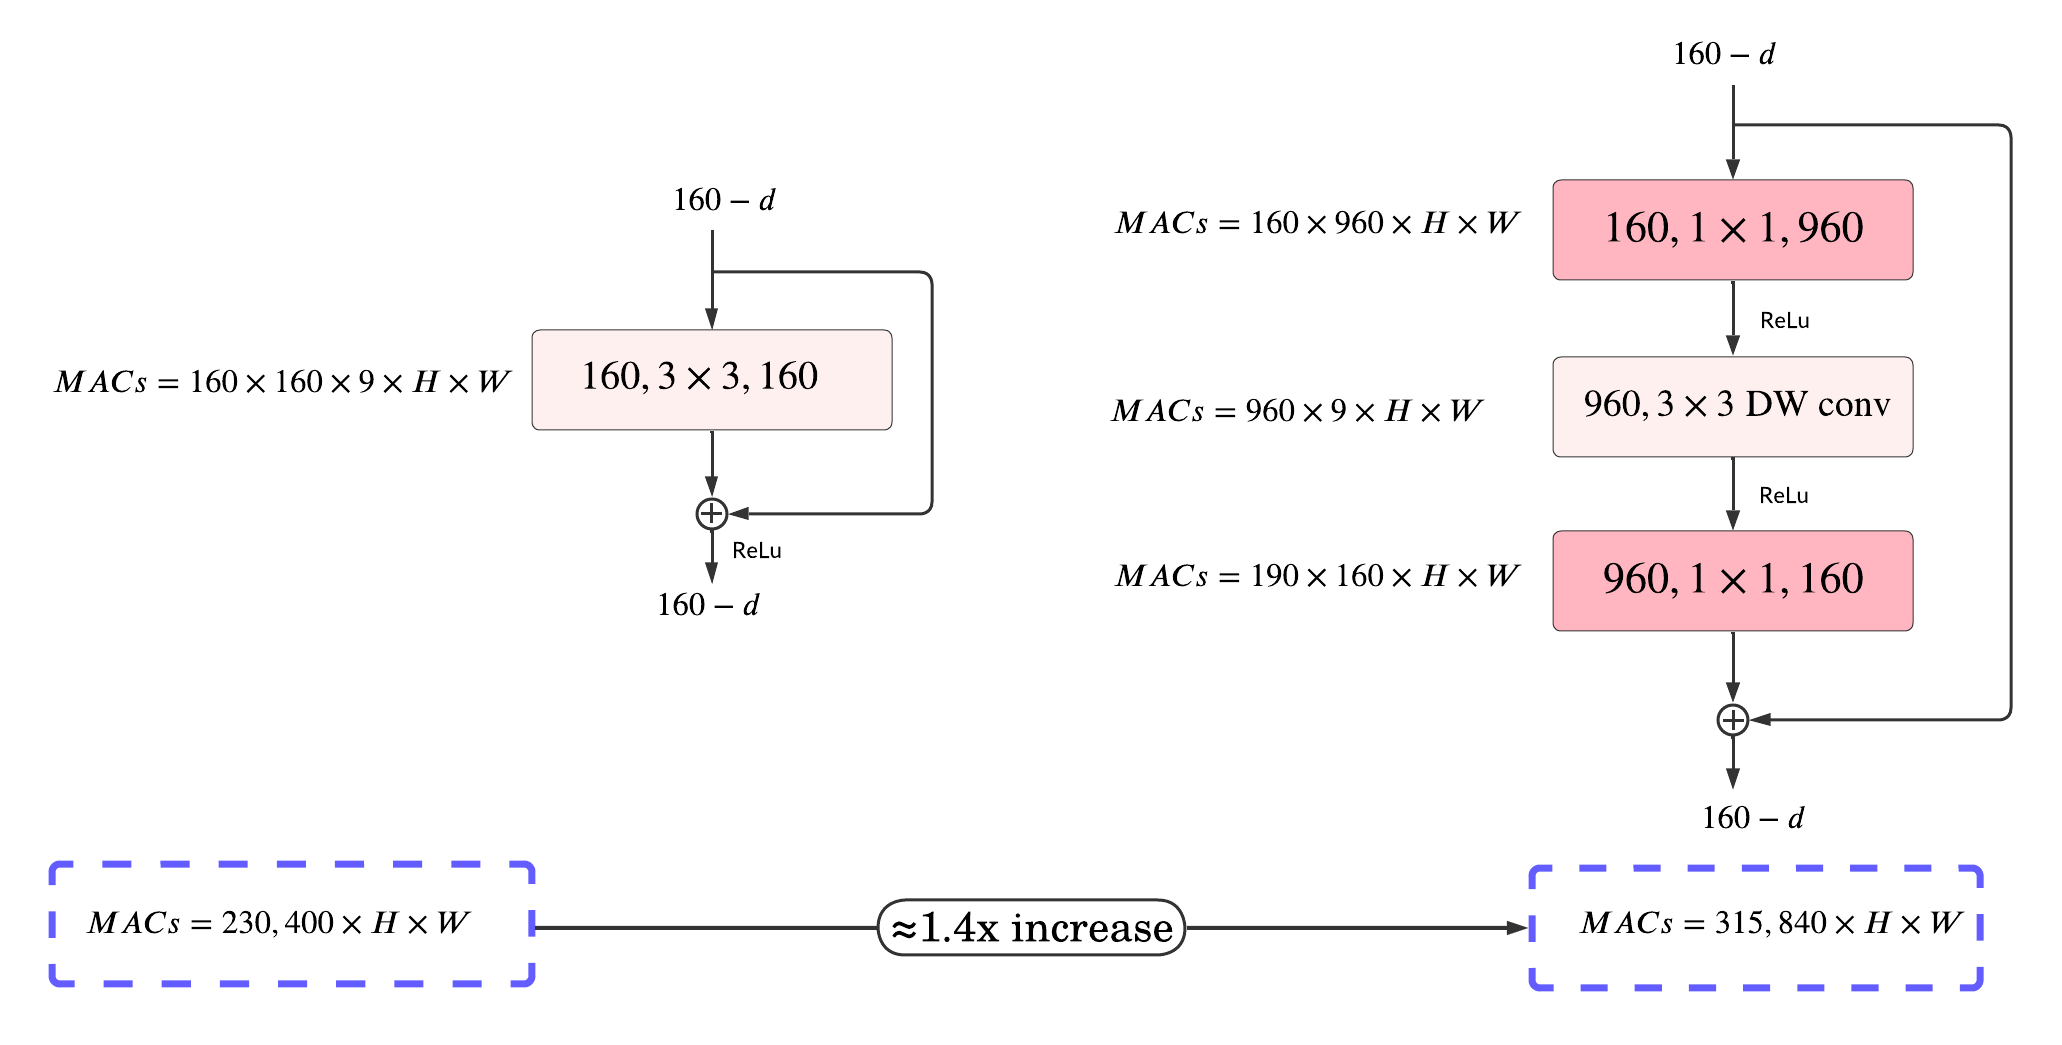
\includegraphics[width=.8\textwidth]{assets/images/inverted.png}
                \end{center}
                \caption{Inverted Bottleneck Residual Block}%
                \label{fig:hw-nas:dl:inverted}
            \end{figure}
            
                    
    
        \subsubsection{ShuffleNet Choice Block}
        
            The ShuffleNet Block is introduced as a part of the ShuffleNet architecture~\cite{mobilenetv2}. It is based on the bottleneck block but establishes some modifications. The block sequence involves a pointwise grouped convolution, followed by a depthwise convolution 3×3, and then another grouped pointwise convolution. 
            Although grouped convolutions reduce computational cost, they can cause information loss because the different groups operate independently and don't exchange information. To address this issue, this block incorporates a shuffle operation after the first grouped pointwise convolution to shuffle information across distinct groups before applying the depthwise \(3\times3\) conv (~\Cref{fig:hw-nas:dl:shuffle}). This shuffle operation is efficient because it doesn't involve any MAC operations.

            \begin{figure}[hbt!]
                \begin{center}
                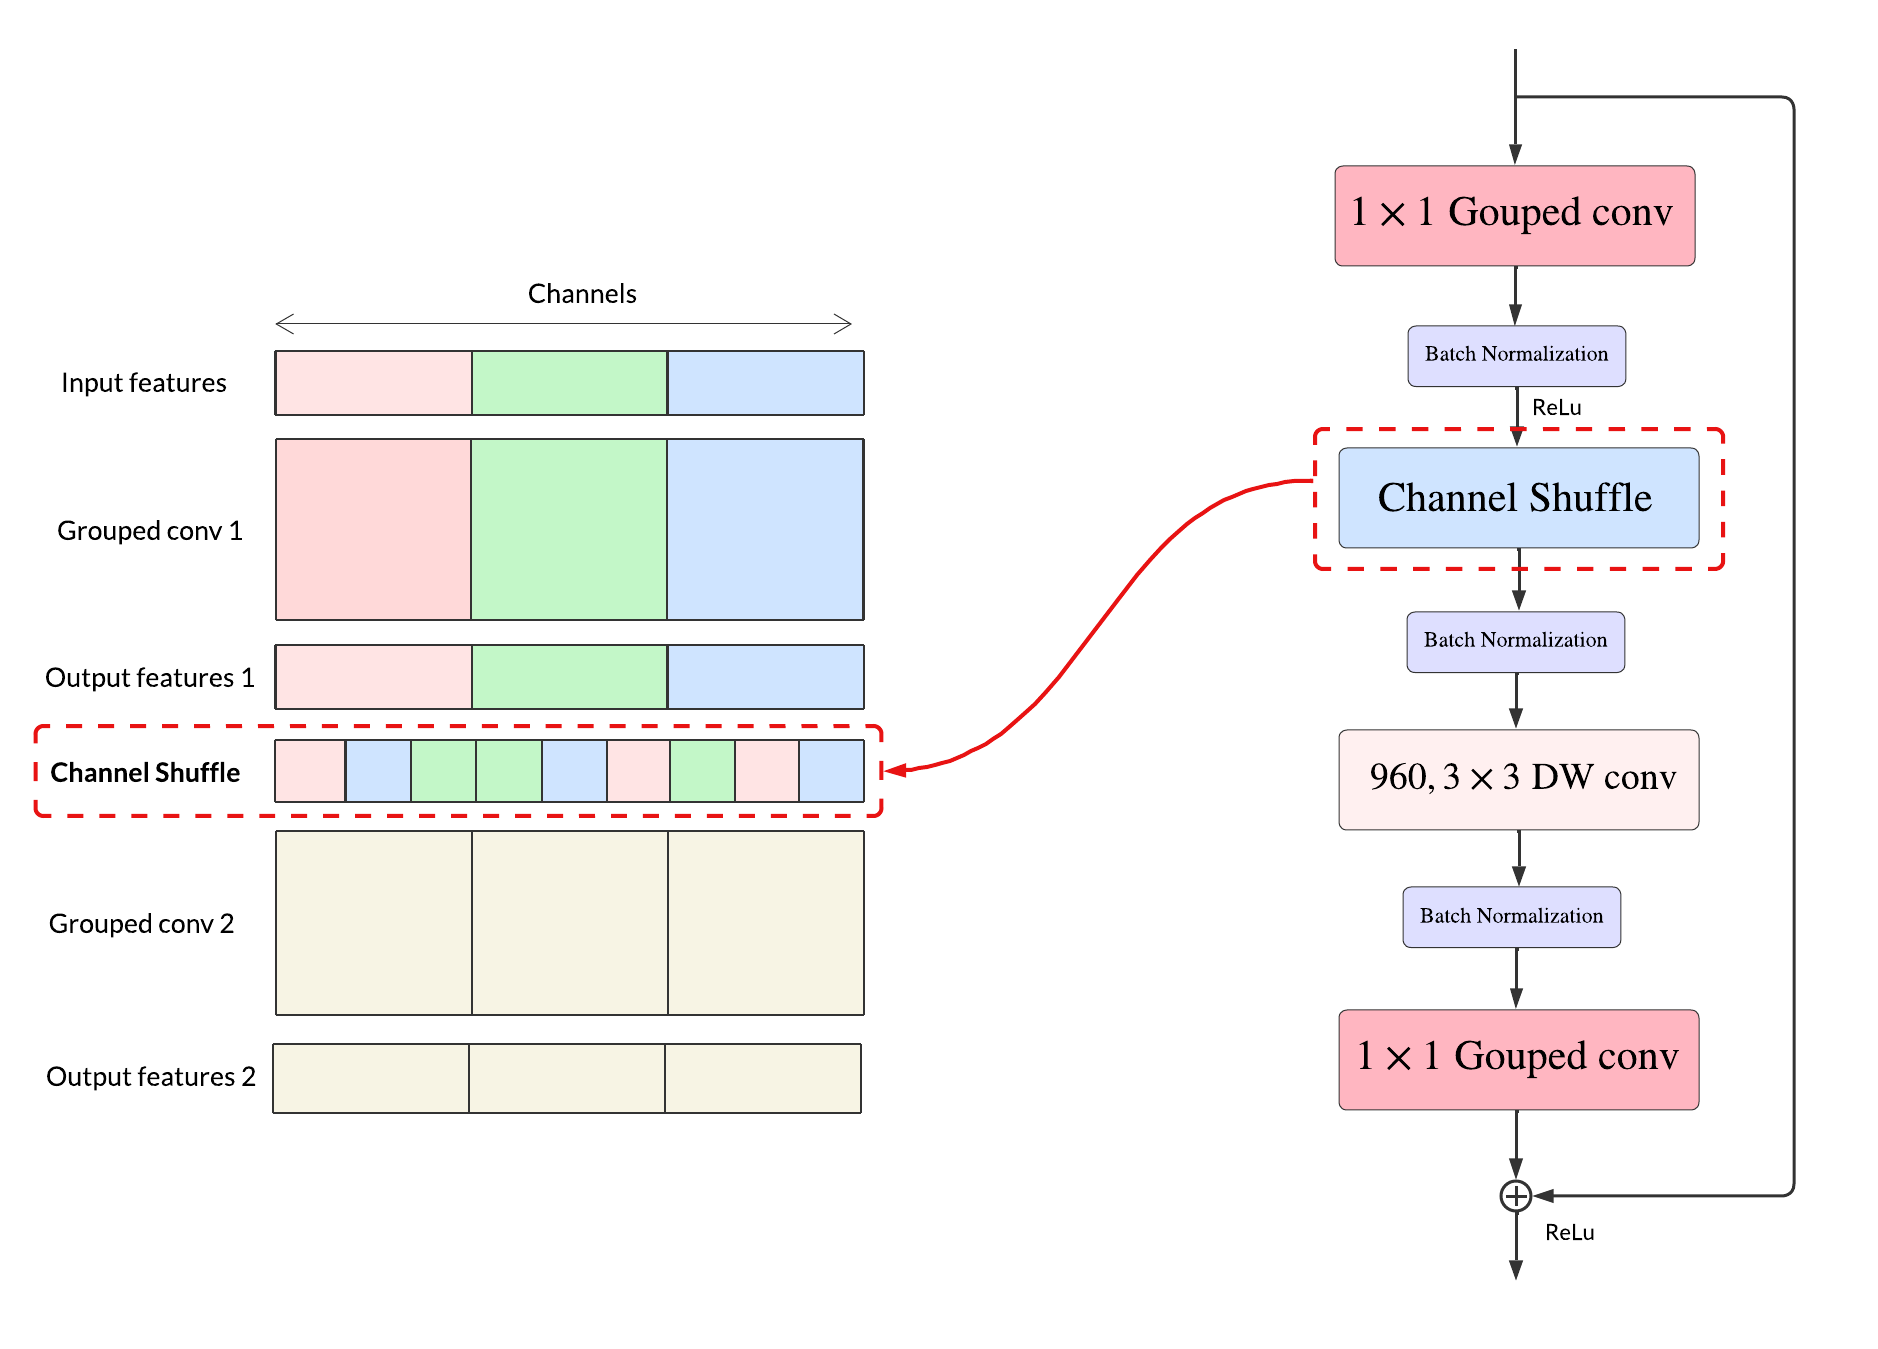
\includegraphics[width=.8\textwidth]{assets/images/shufflenet.png}
                \end{center}
                \caption{ShuffleNet Choice Block}%
                \label{fig:hw-nas:dl:shuffle}
            \end{figure}
            

        
        \subsubsection{Squeeze and Excitation}
        
            \gls{abb:se} block~\cite{squeeze} is a building block designed to enhance the representational power of a \gls{abb:cnn} by adaptively recalibrating channel-wise feature responses through the explicit modeling of interdependencies between channels.
            It consists of a "squeeze" step where each channel is squeezed into a single numeric value using average pooling, followed by an "excitation" step where channel-wise relationships are learned through fully connected layers. The output of the excitation step produces channel-wise scaling factors that are used to re-weight the original feature map channels. 
        
        
        \subsubsection{Multi-head self-attention Block}
    
            Multi-head Attention~\cite{attention} is a block which runs through an attention mechanism several times in parallel. The independent attention outputs are then concatenated and linearly transformed into the expected dimension. 
            The process begins by projecting the input vectors Queries $Q$, Keys $K$, and Values $V$ with $h$ distinct, learned linear projections. Subsequently, the scaled dot-product attention function is executed concurrently on each of these projected versions of $Q$, $K$, and $V$, allowing the model to independently attend to various aspects of the input sequence. The independent attention outputs from these parallel operations are then concatenated and linearly transformed into the expected dimension. 
            

            $MultiHead(Q,K,V) = [head_1, ..,  head_h]W_0$
            
            $\text{where:}\quad  head_i = Attention(Q.W_i^Q, K.W_i^K, V.W_i^V)$
            
